\subsection{SandiaD\_LTS}
%%%%%%%%%%%%%%%%%%%%%%%%%
The \textbf{SandiaD\_LTS} is based on experimental data from Sandia National Laboratories, specifically focusing on turbulent flame dynamics in combustion systems. The turbulent non-premixed Sandia Flame D, studied experimentally by Barlow and Frank~\cite{barlow2005piloted}, is of particular interest as a large amount of data is available for temperature, major species, and pollutant concentrations in the flame and post-flame regions. This configuration was extensively used as a validation case for pollutant formation modelling, as it contains some essential features of turbulence/chemistry interaction

Although the density-based solver developed in this study is fully-compressible, we will show in this section that it is still able to well capture the flow and flame field at Ma = 0.1 − 0.2. The Sandia Flame D piloted partially premixed flame (the maximum Mach number in this flame is about 0.17) is simulated with the TDAC method. Sandia Flame D documentation provides detailed experimental data and the flames are widely validated with different CFD frameworks. Fully compressible solvers is firstly used for Sandia Flame D by Yang et al. with preconditioning scheme. The flow conditions in Sandia Flame D is presented in Table 1. In this study, the current solver is used for the low-speed Sandia Flame D with purpose of testifying the capability of our solve in the low Mach number range. A 2D wedge computational domain is used in this simulation with the Reynolds Averaged transport equations. The Reynolds stress term is closed with the \textbf{standard k − $\epsilon$ model}. Turbulence-chemistry interaction is handles by the \textbf{EDC model}. The chemistry source term integration is achieved
by solving a series of ODE equations, where \textbf{tabulated dynamic adaptive chemistry (TDAC)} is used to accelerate the computation. \textbf{GRI3.0 mechanism} [31] is used for the chemical kinetics.

\subsubsection*{Computational domain and numerical setup}
Present investigation case is Sandia Flame D~\cite{barlow2005piloted} and the burner schematic is shown in Fig.~\ref{fig:domain}. The axisymmetric piloted burner has a main jet inner diameter (D) of 7.2 mm. The pilot annulus inner diameter and outer diameter is 7.7 mm and 18.2 mm, respectively. The burner outer wall diameter is 18.9 mm. Computational domain is a wedge with 5° and its axial and radial length is 80D × 20D. Grid cells around the axis and has a resolution of 162 × 1 × 500. The mesh has a minimum grid of 0.125 mm and a total cell number of 81000. Based on Reynolds numbers of 22 400, air-coow, piloted jet and main fuel jet have bulk inflow velocity of 0.9 m s−1, 11.4 m s−1 and 49.6 m s−1 , and have inflow temperature of 291 K, 1880 K and 294 K, respectively. The velocities of coflow and main fuel jet are under the standard state of 294 K, 0.993 atm. The pilot bulk velocity is estimated from the specified conditions, the flow area of the pilot annulus and the measured mass flow rates. The ambient pressure is 0.996 atm. Fuel is $CH_4$/air mixtures with a volume ratio of 1:3 $\delta$Z ¼ 1. The piloted jet is burned mixtures containing $C_2H_2$, $H_2$, air, $CO_2$ and $N_2$ Z ¼ 0:271. The pressure inlet boundary condition adopts the Neumann condition, and the pressure outlet boundary condition adopts the Dirichlet condition. The inlet boundary condition of other solution variables adopts Dirichlet condition, the outlet boundary condition adopts Neumann condition, and the wall adopts noslip wall condition. Specifically, the $k$ and $\omega$ use the wall function. Periodic boundary conditions are used on the left and right sides.

\begin{figure}[H]
    \centering
    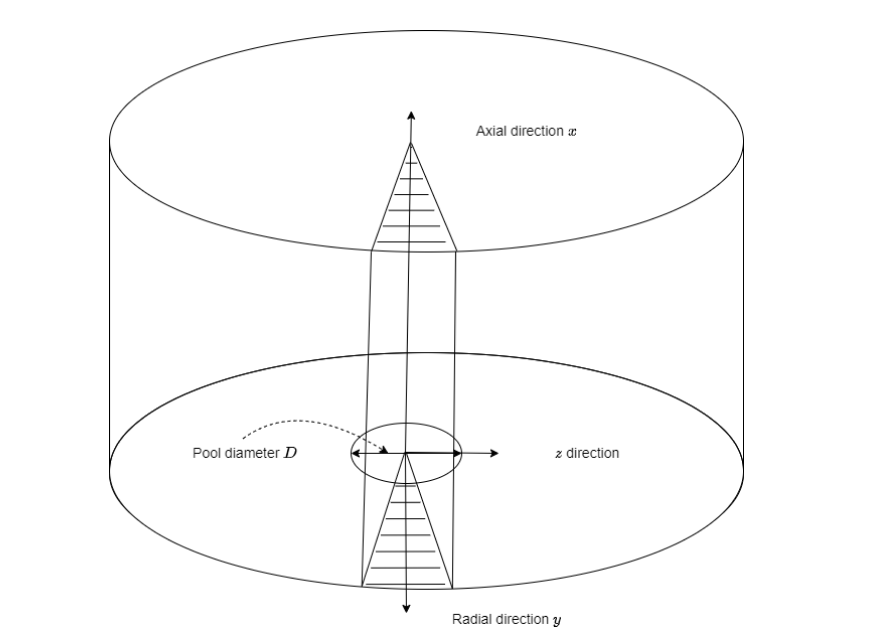
\includegraphics[width=0.95\linewidth]{figs/SandiaD/Screenshot from 2025-03-12 08-14-12.png}
    %\caption{Schematic representation of the numeric domain in the SandiaD LTS tutorial case. Dimensions in mm.}
    \label{fig:domain2}
\end{figure}

\begin{figure}[H]
    \centering
    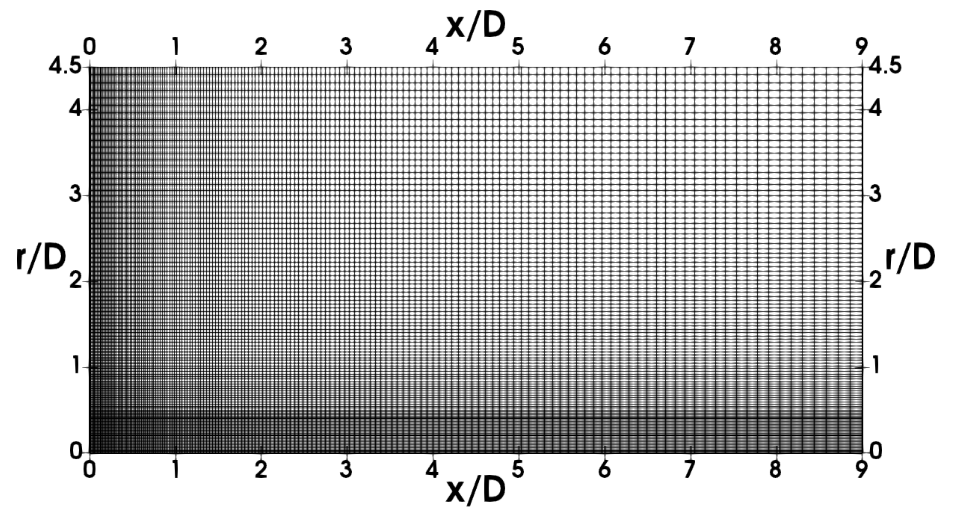
\includegraphics[width=0.95\linewidth]{figs/SandiaD/Screenshot from 2025-03-12 08-14-26.png}
    %\caption{Schematic representation of the numeric domain in the SandiaD LTS tutorial case. Dimensions in mm.}
    \label{fig:domain2}
\end{figure}

\begin{figure}[H]
    \centering
    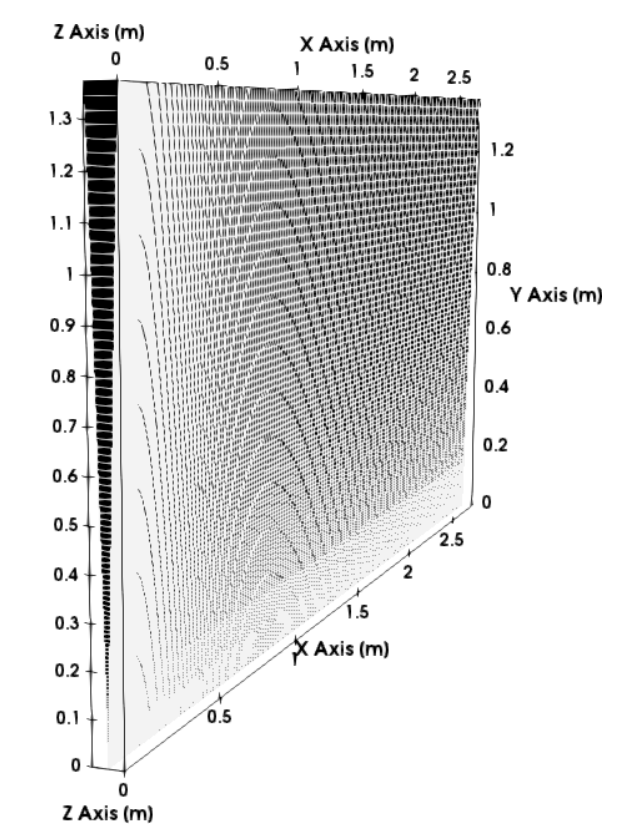
\includegraphics[width=0.65\linewidth]{figs/SandiaD/Screenshot from 2025-03-12 08-15-01.png}
    %\caption{Schematic representation of the numeric domain in the SandiaD LTS tutorial case. Dimensions in mm.}
    \label{fig:domain2}
\end{figure}

\begin{figure}[H]
    \centering
    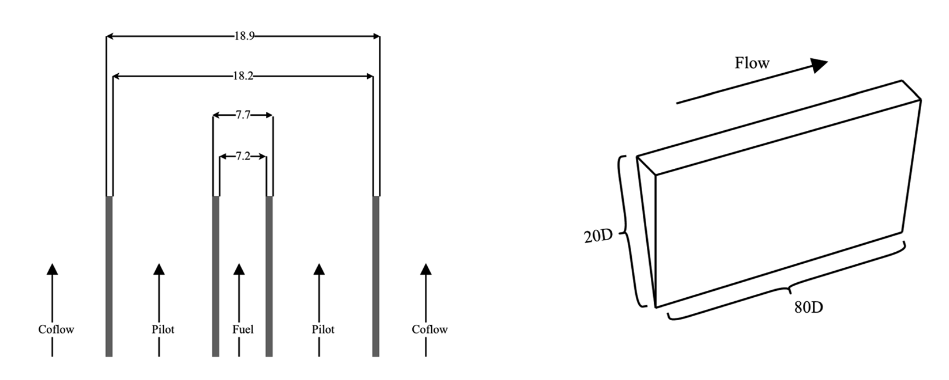
\includegraphics[width=0.95\linewidth]{figs/SandiaD/Screenshot from 2025-03-12 07-11-47.png}
    \caption{The burner schematic in cross section view (a) and axis view (b) of the Sandia Flame D.}
    \label{fig:domain}
\end{figure}

\begin{figure}[H]
    \centering
    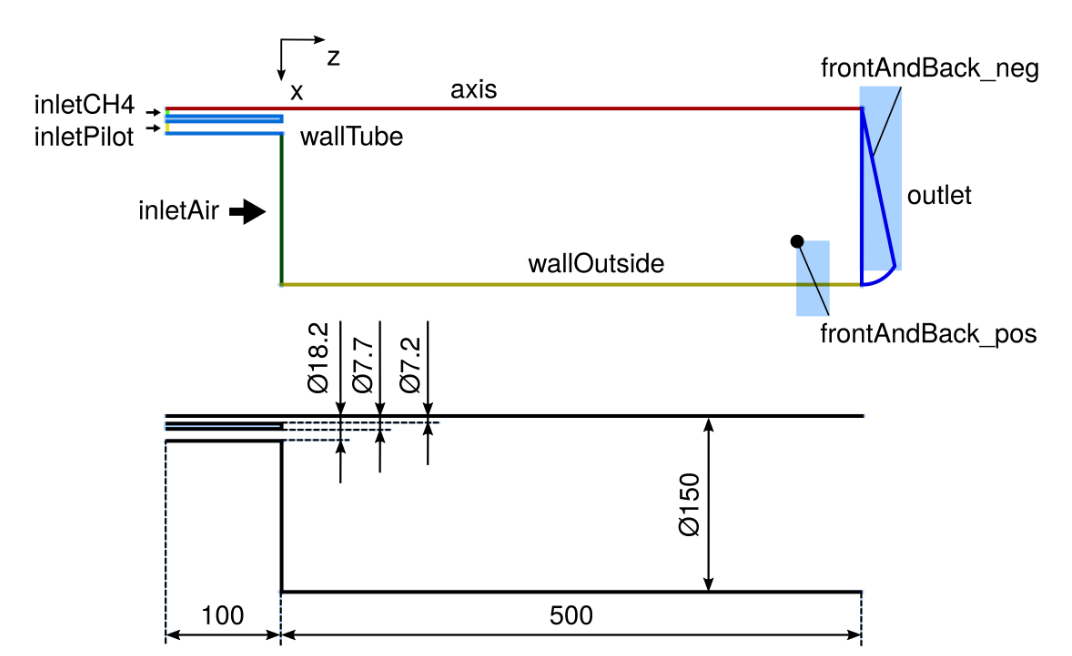
\includegraphics[width=0.95\linewidth]{figs/SandiaD/Screenshot from 2025-03-12 06-58-20.png}
    \caption{Schematic representation of the numeric domain in the SandiaD LTS tutorial case. Dimensions in mm.}
    \label{fig:domain2}
\end{figure}

\subsubsection*{Initial and boundary conditions (0)}
The 0 directory contains pressure $p$, velocity $U$, turbulence kinetic energy $k$, turbulence dissipation rate $\omega$, turbulence viscosity $\nu_t$, and turbulent thermal diffusivity $\alpha_t$. Also, temperature $T$ and incident radiation $G$, as well as the mass fractions of $CO$, $CO_2$, $H$, $H_2$, $H_2O$, $N_2$, $O$, $O_2$ and $OH$. The initial and boundary conditions for the mass fractions of all other included species are set by $Y$default. The computational domain is a wedge representing the axisymmetric setup. The boundaries and dimensions of the domain are shown in Figure~\ref{fig:domain2}. A rich methane-air mixture with 25\% $CH_4$ enters the domain at inletCH4, corresponding to a fuel-air equivalence ratio $\phi$ = 3.17. The diameter of inletCH4 is 7.2 mm. Both inletCH4 and inletPilot are modelled from 100 mm upstream of the expansion to wallOutside. An overview over selected inlet boundary conditions is given in Table~\ref{tab:inlet_boundaries}.

\begin{table}[H]
\centering
\caption{Inner and outer diameter in mm, axial velocity component in m/s, turbulence intensity, mixing length in m, temperature in K, and equivalence ratio at the three inlet boundaries.}
\label{tab:inlet_boundaries}
\adjustbox{max width=\textwidth}{%
\begin{tabular}{cccccccc}
\hline
\textbf{Inlet} & \textbf{$d_i$ (mm)} & \textbf{$D$ (mm)} & \textbf{$U$ (m/s)} & \textbf{Turb. Intensity} & \textbf{Mix. Length (m)} & \textbf{$T$ (K)} & \textbf{$\phi$} \\ \hline
inletCH4       & -                   & 7.2               & 49.6               & 0.0458                  & $5.04 \times 10^{-4}$   & 294              & 3.17            \\ \hline
inletPilot     & 7.7                 & 18.2              & 11.4               & 0.0628                  & $7.35 \times 10^{-4}$   & 1880             & 0.77            \\ \hline
inletAir       & 18.2                & 300               & 0.9                & 0.0471                  & 0.019677                 & 291              & 0               \\ \hline
\end{tabular}}
\end{table}

The lean combustion process of the pilot flame is not solved, instead an inlet condition corresponding the product of the combustion process is prescribed at inletPilot. The inlet temperature at the pilot inlet is set to 1880 K, and the product concentration was calculated separately for a premixed unstrained flame at $\phi$ = 0.77, with the mass fractions of the major species and radicals given in Table~\ref{tab:species_mass_fractions}. At inletAir, air at a temperature of 291 K enters the domain at a speed of 0.9 m/s.

\begin{table}[H]
\centering
\caption{Species mass fractions at the three inlet boundaries.}
\label{tab:species_mass_fractions}
\adjustbox{max width=\textwidth}{%
\begin{tabular}{ccccccccccc}
\hline
\textbf{Inlet} & \textbf{N2} & \textbf{O2} & \textbf{CH4} & \textbf{CO2} & \textbf{H2O} & \textbf{H2} & \textbf{OH} & \textbf{CO} & \textbf{O} & \textbf{H} \\ \hline
inletCH4       & 0.6473      & 0.1966      & 0.1561       & 0            & 0            & 0           & 0           & 0          & 0         & 0        \\ \hline
inletPilot     & 0.7342      & 0.054       & 0            & 0.1098       & 0.0942       & $1.29 \times 10^{-4}$ & $2.8 \times 10^{-3}$ & $4.07 \times 10^{-3}$ & $7.47 \times 10^{-4}$ & $2.48 \times 10^{-5}$ \\ \hline
inletAir       & 0.77        & 0.23        & 0            & 0            & 0            & 0           & 0           & 0          & 0         & 0        \\ \hline
\end{tabular}}
\end{table}

A no-slip condition is specified at wallTube, while zero velocity gradient is specified at wallOutside. Wall functions are applied for both wall patches for $k$, $\omega$ and $nu_t$. The outlet is modelled as a 1e5 Pa total pressure outlet.

\subsubsection*{chemistryProperties.orig}
Under \hl{\texttt{chemistryType}}, the solver \texttt{ode} is selected to solve ordinary differential equations. Tabulation of Dynamic Adaptive Chemistry (TDAC) is chosen as the solution method to speed up chemistry calculations. This feature was added in OpenFOAM-v5. It was demonstrated that this chemistry reduction can increase the efficiency of solving species transport in the case of modestly detailed reaction mechanisms like GRI-Mech 3.0~\cite{ref6}. The initial chemical time step size is set to $1 \times 10^{-7}$ s, which is independent of the flow time step size specified in \texttt{system/controlDict}. 

Under \texttt{odeCoeffs}, the ODE solver \texttt{seulex} is selected, and absolute and relative tolerances are specified. Under \texttt{importantSpecies}, the species which are to be left together with elementary reactions at the end of the reduction process are specified~\cite{ref7}. Finally, the tolerances for reduction and tabulation are specified.

\subsubsection*{combustionProperties}
In this file, the Eddy Dissipation Concept (EDC) turbulent combustion model is selected. Under \hl{\texttt{EDCCoeffs}}, the version of the EDC model is specified, in this tutorial \texttt{v2005}. For this particular version, $C_\gamma = 2.1377$ and $C_\tau = 0.4083$ in:
\begin{equation}
R_i = \rho \frac{\tau^*}{\gamma_L^2 \chi} \frac{1 - \gamma_L^2 \chi}{Y_i - Y_i^*}.
\end{equation}
Here, $R_i$ is the mean reaction rate of species $i$, $\rho$ is the mean density, $\chi$ is the reaction fraction of the fine structures, $Y_i$ is the mean mass fraction of species $i$, and $Y_i^*$ is the fine structure mass fraction of species $i$. Further,
\begin{equation}
\gamma_L = C_\gamma \mathrm{Re}_t^{-1/4}
\end{equation}
is the structure length fraction, and
\begin{equation}
\tau^* = C_\tau \mathrm{Re}_t^{-1/2} \frac{k}{\epsilon}
\end{equation}
denotes the fine structure residence time, based on the turbulent Reynolds number $\mathrm{Re}_t$~\cite{ref8}.

\subsubsection*{radiationProperties}
The model settings for the radiation model are then set in \hl{\texttt{radiationProperties}}.
This file includes a switch to decide whether radiation is considered in the simulation. In the current case, the P1 radiation model is selected. The frequency at which radiation iterations are to be carried out is specified relative to the number of flow iterations. In this tutorial case, it is selected to have one radiation iteration for every single flow iteration. A radiation absorption and emission submodel is specified, in this case \texttt{greyMeanCombustion}. This model gives the radiation and emission coefficients for the continuous phase. Model coefficients need to be supplied for all species that are being solved, i.e., which are not included in a lookup-table for absorption and emission coefficients. 

In this tutorial case, no such lookup-table is used. Instead, the model parameters are supplied in the form of polynomial coefficients for two fifth-order polynomials for a low and a high temperature range. The temperature limit between the low and high temperature regions is also specified. In this tutorial case, only the limit temperature is set to 200 K; therefore, only the coefficients for the high temperature region need to be specified, and the low temperature coefficients are dummy 0 values. In this case, neither scatter nor soot is considered in the radiation absorption and emission submodel.

\subsubsection*{g}
Gravity is taken into account in this testcase. The gravitational acceleration is specified in this file.

\subsubsection*{reactionsGRI}
\textbf{5 elements, 36 species, 218 reactions}, and the valid temperature range are specified in this file.

\subsubsection*{thermo.compressibleGasGRI}
Contains information in OpenFOAM format for 53 species, including molar weight, polynomial coefficients for the specific heat capacity, transport coefficients, and elementary composition.

\subsubsection*{thermophysicalProperties}
Specification of an inert species, in this case $\mathrm{N}_2$. This species is calculated explicitly as $Y_{\text{inert}} = 1 - \sum Y_{\text{active},i}$. The type of chemistry reader, as well as the paths to the above-described chemistry (\texttt{reactionsGRI}) and chemistryThermo (\texttt{thermo.compressibleGasGRI}) files, are specified. Furthermore, seven options in the \texttt{thermoType} package are set:

\begin{itemize}
    \item \textbf{Thermophysical models:} For \texttt{reactingFoam}, the \texttt{hePsiThermo} model class is selected. The \texttt{reactingFoam} solver constructs the model classes \texttt{psiThermo} as well as \texttt{psiReactionThermo}. A fixed composition is assumed, and they are based on the compressibility $\psi = (RT)^{-1}$, where $R$ is the universal gas constant.
    \item \textbf{Mixture model:} For the \texttt{reactingFoam} solver, mixtures with variable composition have to be considered; therefore, the \texttt{reactingMixture} model is selected. This model requires the model coefficients provided in the chemistry file \texttt{reactionsGRI}.
    \item \textbf{Transport model:} One of four transport models is selected. In this case, the Sutherland model is described in the following section.
    \item \textbf{Thermodynamic model:} This model is used to determine the specific heat capacity $c_p$. In this tutorial case, \texttt{janaf} is selected. In this model, $c_p$ is determined based on tabulated coefficients as:
    \begin{equation}
    c_p = R \left( \left( \left( \left( a_4 T + a_3 \right) T + a_2 \right) T + a_1 \right) T + a_0 \right).
    \end{equation}
    \item \textbf{Energy variable:} In this case, the sensible enthalpy $h_s$ is selected as the variable in the energy equation.
    \item \textbf{Equation of state:} In the tutorial case, the perfect gas law:
    \begin{equation}
    \rho = \frac{p}{RT}
    \end{equation}
    is incorporated into the model.
    \item \textbf{Composition:} The keyword \texttt{specie} refers to the submodel describing the molar weight of each species.
\end{itemize}

\subsubsection*{turbulenceProperties}
The RANS model \texttt{kEpsilon} is selected for turbulence modeling. A detailed description of the required files in the \texttt{constant} directory for \texttt{reactingFoam} can be found, for example, in Haddadi et al. 2015~\cite{ref9}.

\subsubsection*{Chemistry and Transport Properties (chemkin)}
In \texttt{constant/thermophysicalModels}, \texttt{sutherland} is specified as the transport model; therefore, the Sutherland coefficient $A_s$ and the Sutherland temperature $T_s$ need to be specified in \texttt{chemkin/transportProperties} for each of the species. The Sutherland model gives the dynamic viscosity as:
\begin{equation}
\mu = A_s \frac{\sqrt{T}}{1 + \frac{T_s}{T}},
\end{equation}
where $T$ is the variable temperature. This transport model also gives the thermal conductivity $\kappa$ and the thermal diffusivity $\alpha$. $A_s = 1.512 \times 10^{-6} \, \mathrm{Pa \, s \, K^{-0.5}}$ and $T_s = 120 \, \mathrm{K}$ are specified for all species but $\mathrm{H}_2$ and $\mathrm{CO}_2$, for which the model parameters are set individually.

The \texttt{grimech30.dat} file contains the description of the reaction mechanisms with corresponding rate constants, altogether 325 reactions for 53 species. \texttt{Thermo30.dat} contains the corresponding thermochemical data, in the form of NASA polynomial coefficients for each species. The utility \texttt{chemkinToFoam} converts the three files, \texttt{grimech30.dat} and \texttt{thermo30.dat} in chemkin-II format, and \texttt{transportProperties}, to \texttt{reactionsGRI} and \texttt{thermo.compressibleGasGRI} in the \texttt{constant} directory.

\subsubsection*{Solution Settings (system)}
In \texttt{system/fvSchemes}, the divergence schemes for the transport of species mass fractions $Y_i$ and species enthalpy $Y_i h$ are set. The \texttt{'01'} in \texttt{limitedLinear01} assures stronger bounding between 0 and 1.

\section*{Results}
\begin{figure}[H]
    \centering
    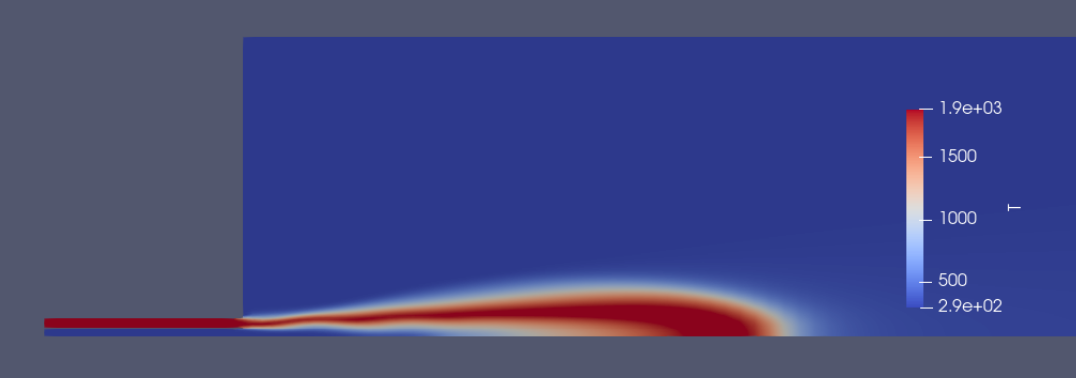
\includegraphics[width=0.95\linewidth]{figs/SandiaD/Screenshot from 2025-03-12 06-59-03.png}
    %\caption{The burner schematic in cross section view (a) and axis view (b) of the Sandia Flame D}
    \label{fig:domain}
\end{figure}

\begin{figure}[H]
    \centering
    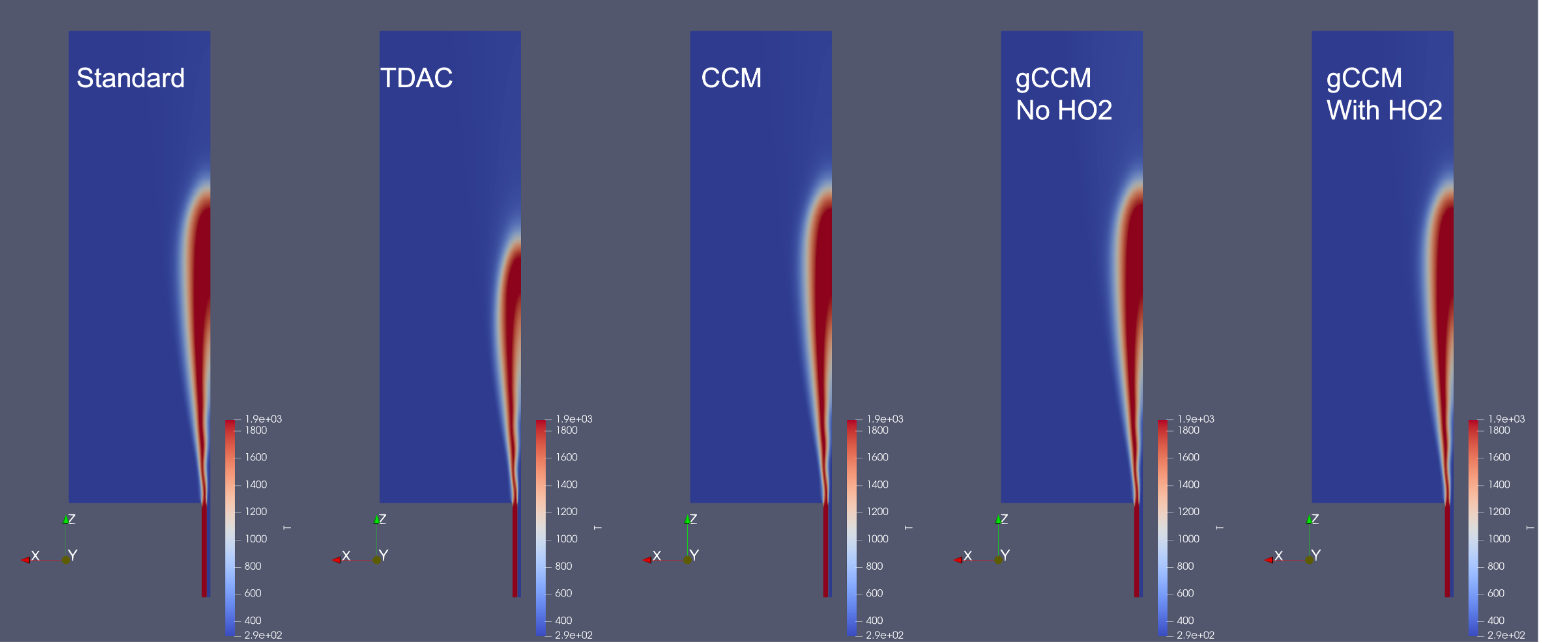
\includegraphics[width=0.95\linewidth]{figs/SandiaD/Screenshot from 2025-03-12 06-59-49.png}
    %\caption{The burner schematic in cross section view (a) and axis view (b) of the Sandia Flame D}
    \label{fig:domain}
\end{figure}

\begin{figure}[H]
    \centering
    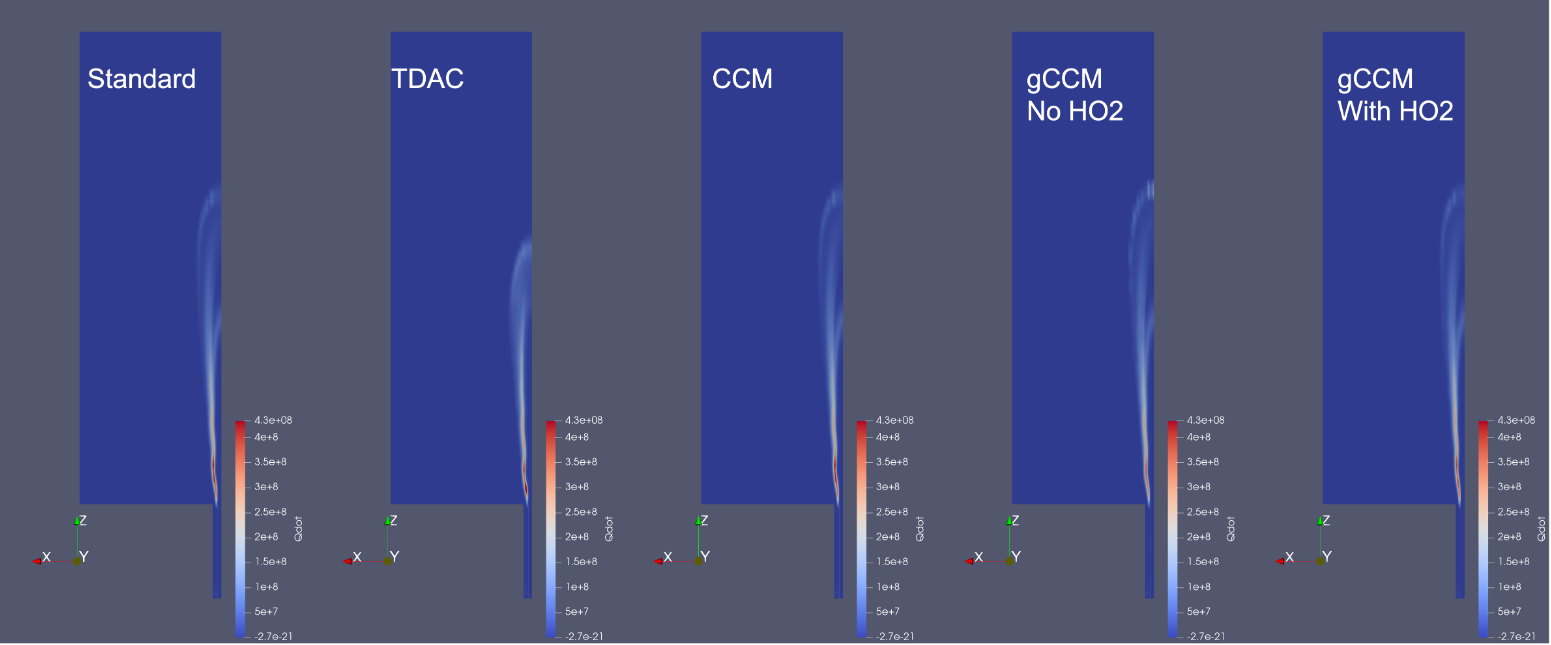
\includegraphics[width=0.95\linewidth]{figs/SandiaD/Screenshot from 2025-03-12 07-00-20.png}
    %\caption{The burner schematic in cross section view (a) and axis view (b) of the Sandia Flame D}
    \label{fig:domain}
\end{figure}

\begin{figure}[H]
    \centering
    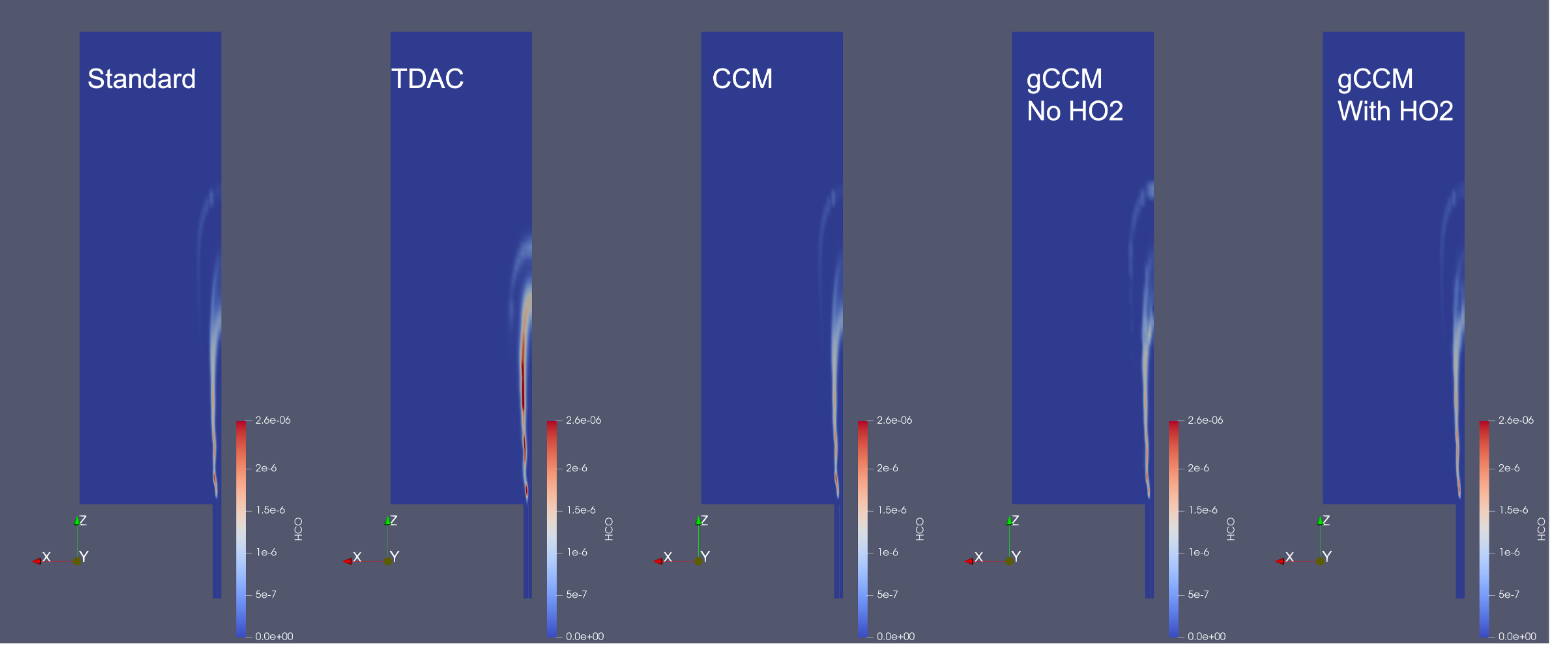
\includegraphics[width=0.95\linewidth]{figs/SandiaD/Screenshot from 2025-03-12 07-00-42.png}
    %\caption{The burner schematic in cross section view (a) and axis view (b) of the Sandia Flame D}
    \label{fig:domain}
\end{figure}

\begin{figure}[H]
    \centering
    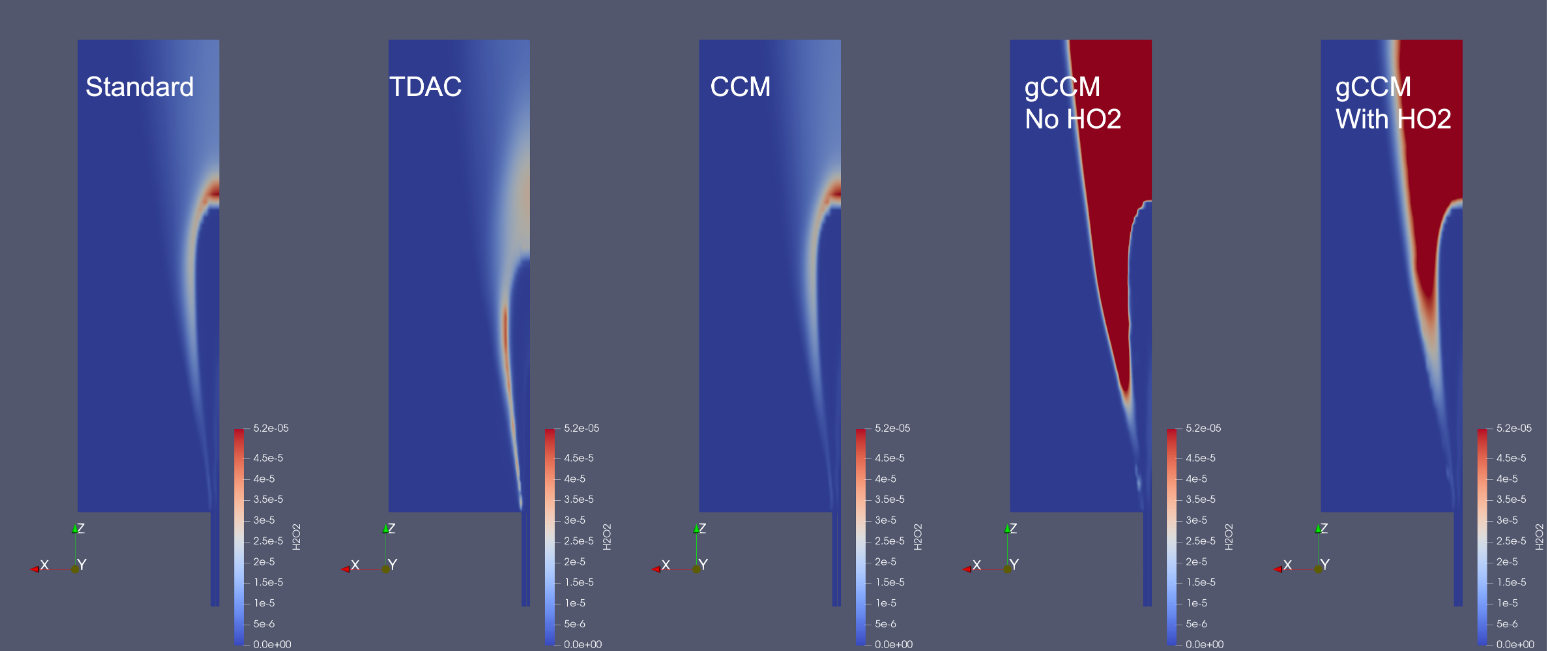
\includegraphics[width=0.95\linewidth]{figs/SandiaD/Screenshot from 2025-03-12 07-01-10.png}
    %\caption{The burner schematic in cross section view (a) and axis view (b) of the Sandia Flame D}
    \label{fig:domain}
\end{figure}

\begin{figure}[H]
    \centering
    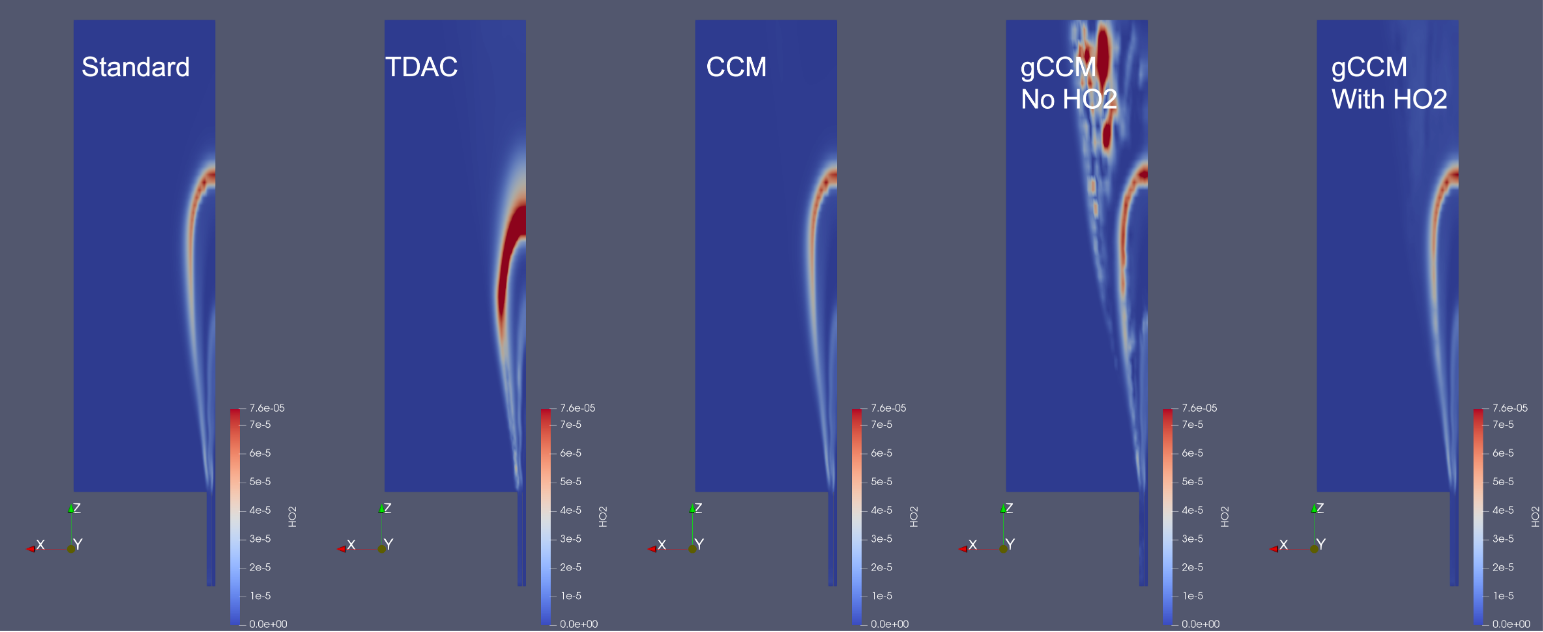
\includegraphics[width=0.95\linewidth]{figs/SandiaD/Screenshot from 2025-03-12 07-01-27.png}
    %\caption{The burner schematic in cross section view (a) and axis view (b) of the Sandia Flame D}
    \label{fig:domain}
\end{figure}

\begin{figure}[H]
    \centering
    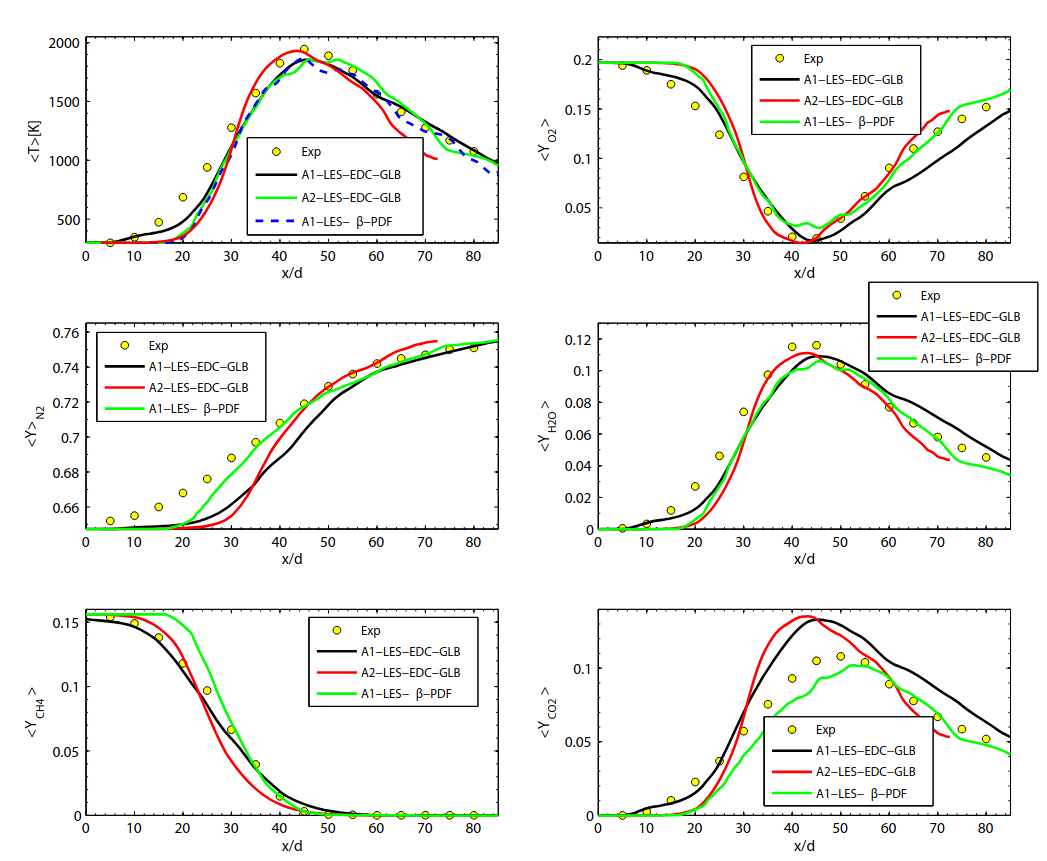
\includegraphics[width=0.95\linewidth]{figs/SandiaD/Screenshot from 2025-03-12 06-57-30.png}
    %\caption{The burner schematic in cross section view (a) and axis view (b) of the Sandia Flame D}
    \label{fig:domain}
\end{figure}

\begin{figure}[H]
    \centering
    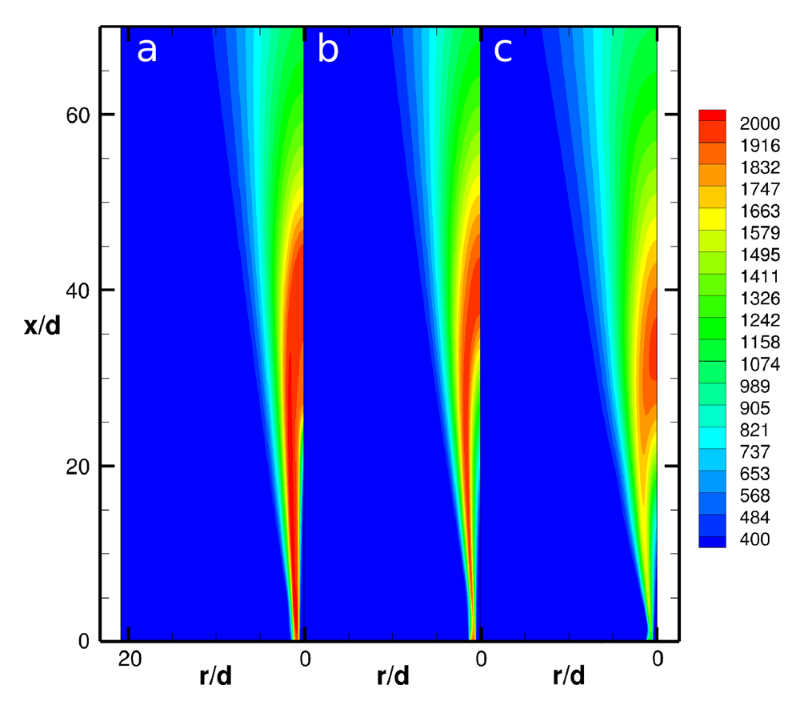
\includegraphics[width=0.95\linewidth]{figs/SandiaD/Screenshot from 2025-03-12 06-55-33.png}
    %\caption{The burner schematic in cross section view (a) and axis view (b) of the Sandia Flame D}
    \label{fig:domain}
\end{figure}

\begin{figure}[H]
    \centering
    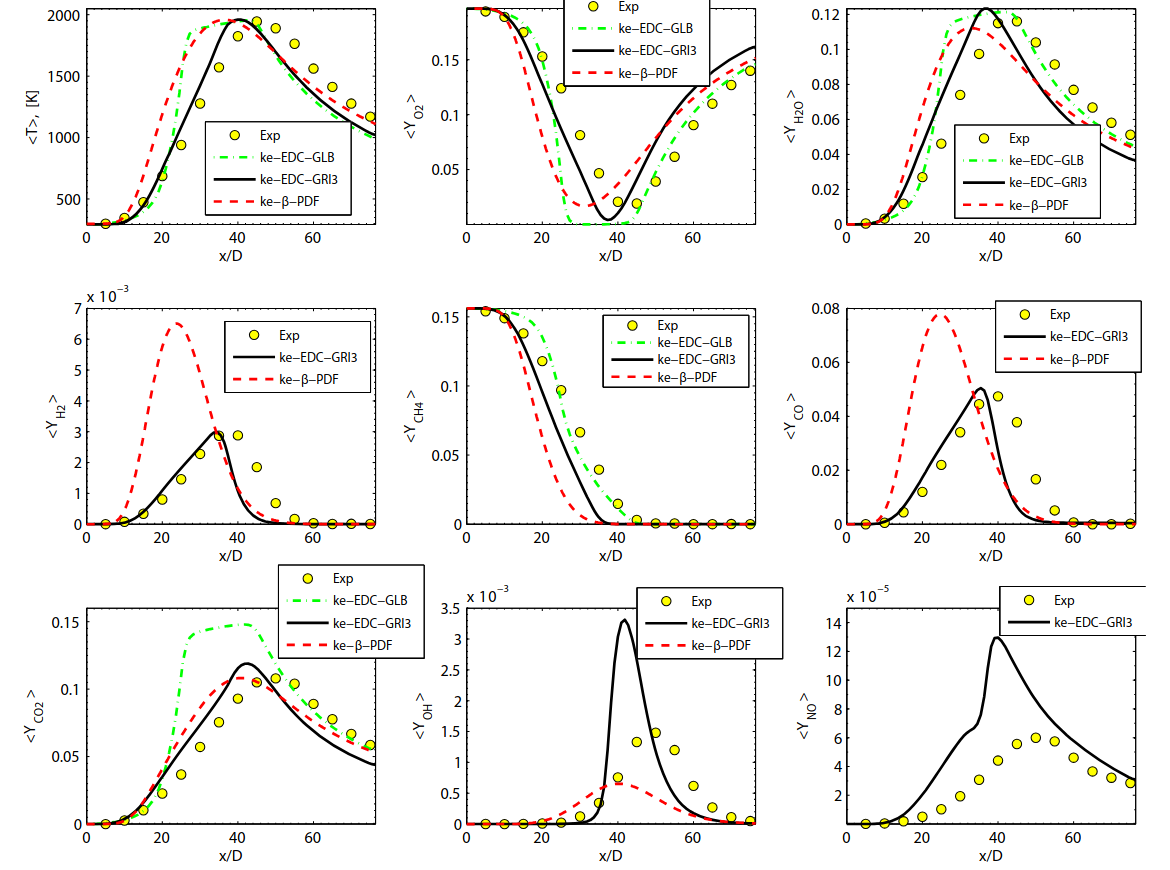
\includegraphics[width=0.95\linewidth]{figs/SandiaD/Screenshot from 2025-03-12 06-56-07.png}
    %\caption{The burner schematic in cross section view (a) and axis view (b) of the Sandia Flame D}
    \label{fig:domain}
\end{figure}

\begin{figure}[H]
    \centering
    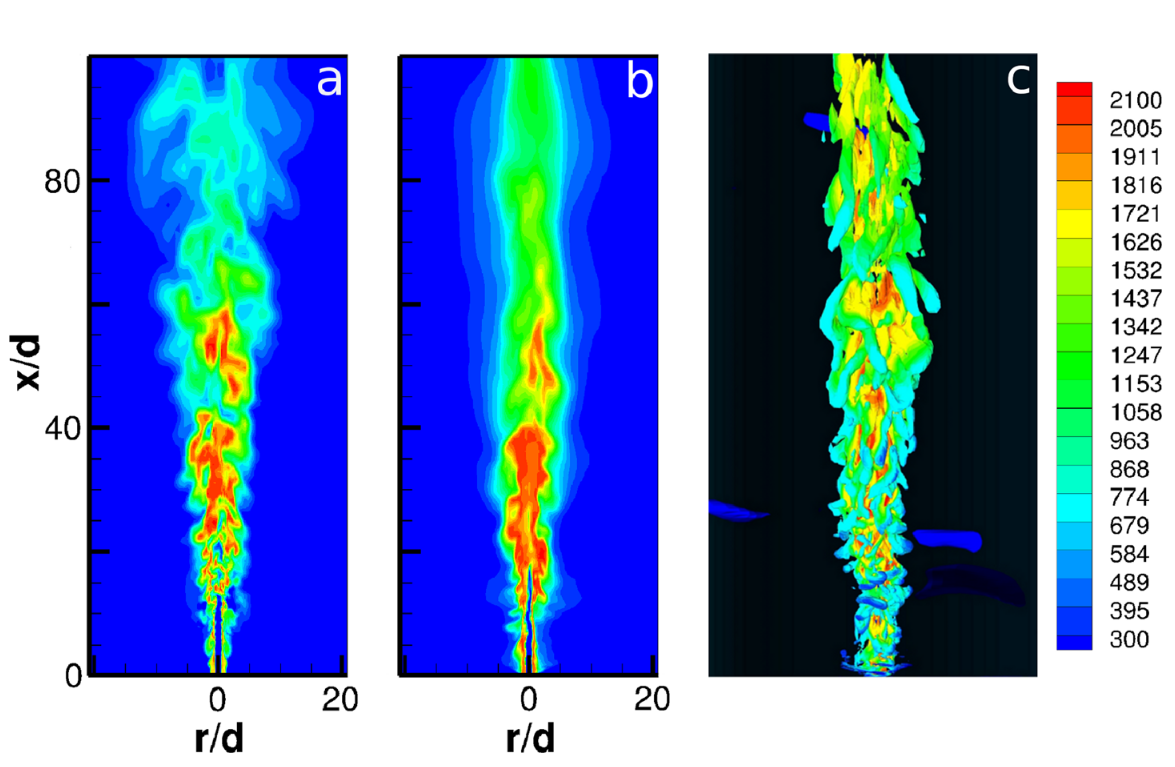
\includegraphics[width=0.95\linewidth]{figs/SandiaD/Screenshot from 2025-03-12 06-56-38.png}
    %\caption{The burner schematic in cross section view (a) and axis view (b) of the Sandia Flame D}
    \label{fig:domain}
\end{figure}

\begin{figure}[H]
    \centering
    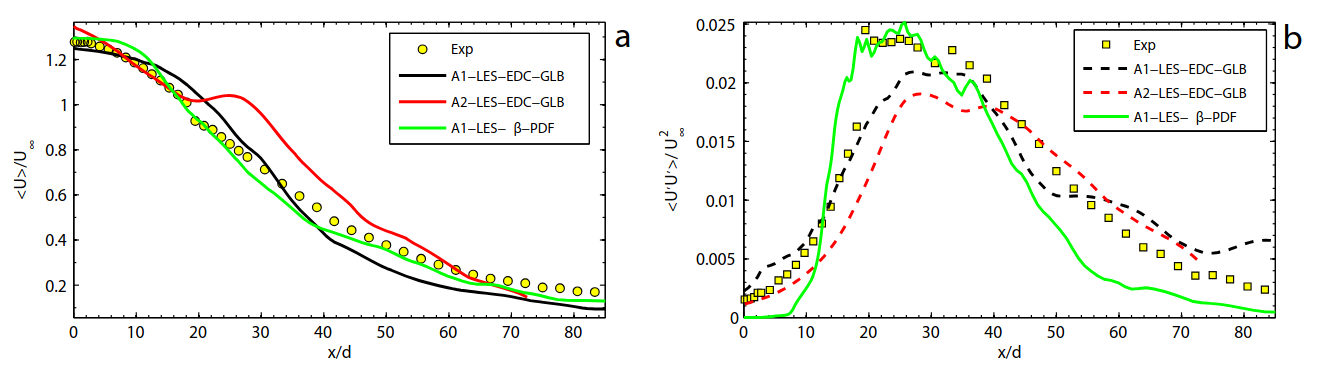
\includegraphics[width=0.95\linewidth]{figs/SandiaD/Screenshot from 2025-03-12 06-57-11.png}
    %\caption{The burner schematic in cross section view (a) and axis view (b) of the Sandia Flame D}
    \label{fig:domain}
\end{figure}

\begin{itemize}
    \item The test case models a turbulent premixed flame, which is a canonical problem in combustion research.
    \item It is derived from the Sandia Flame D experiments, involving methane-air combustion under well-defined conditions.
    \item The flame is stabilized by a bluff-body burner, creating a recirculation zone that stabilizes the flame.
\end{itemize}

%\subsection{Governing Equations}
\begin{itemize}
    \item The simulation solves the \textbf{Reynolds-Averaged Navier-Stokes (RANS)} equations coupled with a combustion model.
    \item A turbulence model, such as the \textbf{k-$\varepsilon$} or \textbf{k-$\omega$ SST} model, is typically used to account for turbulence effects.
    \item Combustion chemistry is modeled using simplified mechanisms, such as the \textbf{Eddy Dissipation Model (EDM)} or \textbf{Finite Rate Chemistry}.
\end{itemize}

\subsubsection*{OpenFOAM Chemistry Properties File}

Below is an example of an OpenFOAM \texttt{chemistryProperties} file:

\begin{lstlisting}[language=C++, caption={chemistryProperties}]
/*--------------------------------*- C++ -*----------------------------------*\
| =========                 |                                                 |
| \\      /  F ield         | OpenFOAM: The Open Source CFD Toolbox           |
|  \\    /   O peration     | Version:  2306                                  |
|   \\  /    A nd           | Website:  www.openfoam.com                      |
|    \\/     M anipulation  |                                                 |
\*---------------------------------------------------------------------------*/
// * * * * * * * * * * * * * * * * * * * * * * * * * * * * * * * * * * * * * //
FoamFile
{
    version         2;
    format          ascii;
    class           dictionary;
    object          chemistryProperties;
}

chemistryType
{
    solver          ode;
    method          TDAC;
}

chemistry       on;

importantSpecies
{
    CO2             ;
    H2O             ;
    CH4             ;
    O2              ;
}

initialChemicalTimeStep 1e-07;

odeCoeffs
{
    solver          seulex;
    absTol          1e-12;
    relTol          1e-07;
}

reduction
{
    active          on;
    log             on;
    tolerance       0.0001;
    method          DAC;
    initialSet
    {
        CO              ;
        CH4             ;
        HO2             ;
    }
    automaticSIS    off;
    fuelSpecies
    {
        CH4             1;
    }
}

tabulation
{
    active          on;
    log             on;
    printProportion off;
    printNumRetrieve off;
    tolerance       0.003;
    method          ISAT;
    scaleFactor
    {
        otherSpecies    1;
        Temperature     10000;
        Pressure        1e+15;
        deltaT          1;
    }
    maxNLeafs       5000;
    chPMaxLifeTime  1000;
    maxGrowth       100;
    checkEntireTreeInterval 500;
    maxDepthFactor  2;
    minBalanceThreshold 30;
    MRURetrieve     false;
    maxMRUSize      0;
    growPoints      true;
    maxNumNewDim    10;
}

// ************************************************************************* //
\end{lstlisting}

%\section*{OpenFOAM Combustion Properties File}

Below is an example of an OpenFOAM \texttt{combustionProperties} file:

\begin{lstlisting}[language=C++, caption={combustionProperties}]
/*--------------------------------*- C++ -*----------------------------------*\
| =========                 |                                                 |
| \\      /  F ield         | OpenFOAM: The Open Source CFD Toolbox           |
|  \\    /   O peration     | Version:  v2306                                 |
|   \\  /    A nd           | Website:  www.openfoam.com                      |
|    \\/     M anipulation  |                                                 |
\*---------------------------------------------------------------------------*/
FoamFile
{
    version     2.0;
    format      ascii;
    class       dictionary;
    object      combustionProperties;
}
// * * * * * * * * * * * * * * * * * * * * * * * * * * * * * * * * * * * * * //

combustionModel  EDC;

active  true;

EDCCoeffs
{
    version v2005;
}

// ************************************************************************* //
\end{lstlisting}

%\section*{OpenFOAM Radiation Properties File}

Below is an example of an OpenFOAM \texttt{radiationProperties} file:

\begin{lstlisting}[language=C++, caption={radiationProperties}]
/*--------------------------------*- C++ -*----------------------------------*\
| =========                 |                                                 |
| \\      /  F ield         | OpenFOAM: The Open Source CFD Toolbox           |
|  \\    /   O peration     | Version:  v2306                                 |
|   \\  /    A nd           | Website:  www.openfoam.com                      |
|    \\/     M anipulation  |                                                 |
\*---------------------------------------------------------------------------*/
FoamFile
{
    version     2.0;
    format      ascii;
    class       dictionary;
    object      radiationProperties;
}
// * * * * * * * * * * * * * * * * * * * * * * * * * * * * * * * * * * * * * //

radiation on;

radiationModel  P1;

P1Coeffs
{
    C               C [0 0 0 0 0 0 0] 0;
}

// Number of flow iterations per radiation iteration
solverFreq 1;

absorptionEmissionModel greyMeanAbsorptionEmission;

greyMeanAbsorptionEmissionCoeffs
{
    lookUpTableFileName      none;

    EhrrCoeff                0.0;

    CO2
    {
        Tcommon         200;   //Common Temp
        invTemp         true;   //Is the polynomio using inverse temperature.
        Tlow            200;   //Low Temp
        Thigh           2500;  //High Temp

        loTcoeffs       //coefss for T < Tcommon
        (
            0           //  a0            +
            0           //  a1*T          +
            0           //  a2*T^(+/-)2   +
            0           //  a3*T^(+/-)3   +
            0           //  a4*T^(+/-)4   +
            0           //  a5*T^(+/-)5   +
        );
        hiTcoeffs        //coefss for T > Tcommon
        (
            18.741
            -121.31e3
            273.5e6
            -194.05e9
            56.31e12
            -5.8169e15
        );

    }

    H2O
    {
        Tcommon         200;
        invTemp         true;
        Tlow            200;
        Thigh           2500;

        loTcoeffs
        (
            0
            0
            0
            0
            0
            0
        );
        hiTcoeffs
        (
            -0.23093
            -1.12390e3
             9.4153e6
            -2.99885e9
             0.51382e12
            -1.868e10
        );
    }

    CH4
    {
        Tcommon         200;
        Tlow            200;
        Thigh           2500;
        invTemp         false;

        loTcoeffs
        (
            0
            0
            0
            0
            0
            0
        );
        hiTcoeffs
        (
            6.6334
            -0.0035686
            1.6682e-8
            2.5611e-10
            -2.6558e-14
            0
        );
    }

    O2
    {
        Tcommon         200;
        invTemp         true;
        Tlow            200;
        Thigh           2500;

        loTcoeffs
        (
            0
            0
            0
            0
            0
            0
        );
        hiTcoeffs
        (
            0.1
            0
            0
            0
            0
            0
        );
    }


    N2
    {
        Tcommon         200;
        invTemp         true;
        Tlow            200;
        Thigh           2500;

        loTcoeffs
        (
            0
            0
            0
            0
            0
            0
        );
        hiTcoeffs
        (
            0.1
            0
            0
            0
            0
            0
        );
    }
}

scatterModel    none;

sootModel       none;

transmissivityModel none;

// ************************************************************************* //
\end{lstlisting}

\begin{lstlisting}[language=C++, caption={boundaryRadiationProperties}]
/*--------------------------------*- C++ -*----------------------------------*\
| =========                 |                                                 |
| \\      /  F ield         | OpenFOAM: The Open Source CFD Toolbox           |
|  \\    /   O peration     | Version:  v2306                                 |
|   \\  /    A nd           | Website:  www.openfoam.com                      |
|    \\/     M anipulation  |                                                 |
\*---------------------------------------------------------------------------*/
FoamFile
{
    version     2.0;
    format      ascii;
    class       dictionary;
    object      boundaryRadiationProperties;
}
// * * * * * * * * * * * * * * * * * * * * * * * * * * * * * * * * * * * * * //

".*"
{
    type            lookup;
    emissivity      1;
    absorptivity    0;
}

// ************************************************************************* //
\end{lstlisting}                                                                  

%\section*{OpenFOAM Thermophysical Properties File}

Below is the thermophysical properties configuration file used in OpenFOAM simulations:

\begin{lstlisting}[language=C++, caption={Thermophysical Properties File}]
/*--------------------------------*- C++ -*----------------------------------*\
| =========                 |                                                 |
| \\      /  F ield         | OpenFOAM: The Open Source CFD Toolbox           |
|  \\    /   O peration     | Version:  v2306                                 |
|   \\  /    A nd           | Website:  www.openfoam.com                      |
|    \\/     M anipulation  |                                                 |
\*---------------------------------------------------------------------------*/
FoamFile
{
    version     2.0;
    format      ascii;
    class       dictionary;
    object      thermophysicalProperties;
}
// * * * * * * * * * * * * * * * * * * * * * * * * * * * * * * * * * * * * * //

thermoType
{
    type            hePsiThermo;
    mixture         reactingMixture;
    transport       sutherland;
    thermo          janaf;
    energy          sensibleEnthalpy;
    equationOfState perfectGas;
    specie          specie;
}

inertSpecie N2;

chemistryReader foamChemistryReader;
foamChemistryFile "<constant>/reactionsGRI";
foamChemistryThermoFile "<constant>/thermo.compressibleGasGRI";

// ************************************************************************* //
\end{lstlisting}

\subsection*{OpenFOAM Radiation Properties File}
%%%%%%%%%%%%%%%%%%%%%%%%%%%%%%%%%%%%%%%%%%%%%
Then, radiationProperties and boundaryRadiationProperties are required to specify the radiation model’s properties. The radiationProperties is a dictionary that specifies the RTE solver and the spectral model under the constant folder, while the boundaryRadiationProperties is a dictionary that specifies the radiation model’s properties on the boundary. The radiationProperties is defined as below, which shows how to select P1 as the RTE solver and the grey mean absorption emission model as the spectral model. The absorption coefficient for each gas is the function of
temperature and is described as a polynomial. 

Below is an example of an OpenFOAM \texttt{radiationProperties} file:\\
\adjustbox{max width=\textwidth}{%
\begin{lstlisting}[language=C++, caption={radiationProperties}]
/*--------------------------------*- C++ -*----------------------------------*\
| =========                 |                                                 |
| \\      /  F ield         | OpenFOAM: The Open Source CFD Toolbox           |
|  \\    /   O peration     | Version:  v2306                                 |
|   \\  /    A nd           | Website:  www.openfoam.com                      |
|    \\/     M anipulation  |                                                 |
\*---------------------------------------------------------------------------*/
FoamFile
{
    version     2.0;
    format      ascii;
    class       dictionary;
    object      radiationProperties;
}
// * * * * * * * * * * * * * * * * * * * * * * * * * * * * * * * * * * * * * //

radiation on;

radiationModel  P1;

P1Coeffs
{
    C               C [0 0 0 0 0 0 0] 0;
}

// Number of flow iterations per radiation iteration
solverFreq 1;

absorptionEmissionModel greyMeanAbsorptionEmission;

greyMeanAbsorptionEmissionCoeffs
{
    lookUpTableFileName      none;

    EhrrCoeff                0.0;

    CO2
    {
        Tcommon         200;   //Common Temp
        invTemp         true;   //Is the polynomio using inverse temperature.
        Tlow            200;   //Low Temp
        Thigh           2500;  //High Temp

        loTcoeffs       //coefss for T < Tcommon
        (
            0           //  a0            +
            0           //  a1*T          +
            0           //  a2*T^(+/-)2   +
            0           //  a3*T^(+/-)3   +
            0           //  a4*T^(+/-)4   +
            0           //  a5*T^(+/-)5   +
        );
        hiTcoeffs        //coefss for T > Tcommon
        (
            18.741
            -121.31e3
            273.5e6
            -194.05e9
            56.31e12
            -5.8169e15
        );

    }

    H2O
    {
        Tcommon         200;
        invTemp         true;
        Tlow            200;
        Thigh           2500;

        loTcoeffs
        (
            0
            0
            0
            0
            0
            0
        );
        hiTcoeffs
        (
            -0.23093
            -1.12390e3
             9.4153e6
            -2.99885e9
             0.51382e12
            -1.868e10
        );
    }

    CH4
    {
        Tcommon         200;
        Tlow            200;
        Thigh           2500;
        invTemp         false;

        loTcoeffs
        (
            0
            0
            0
            0
            0
            0
        );
        hiTcoeffs
        (
            6.6334
            -0.0035686
            1.6682e-8
            2.5611e-10
            -2.6558e-14
            0
        );
    }

    O2
    {
        Tcommon         200;
        invTemp         true;
        Tlow            200;
        Thigh           2500;

        loTcoeffs
        (
            0
            0
            0
            0
            0
            0
        );
        hiTcoeffs
        (
            0.1
            0
            0
            0
            0
            0
        );
    }


    N2
    {
        Tcommon         200;
        invTemp         true;
        Tlow            200;
        Thigh           2500;

        loTcoeffs
        (
            0
            0
            0
            0
            0
            0
        );
        hiTcoeffs
        (
            0.1
            0
            0
            0
            0
            0
        );
    }
}

scatterModel    none;

sootModel       none;

transmissivityModel none;

// ************************************************************************* //
\end{lstlisting}}

For the boundaryRadiationProperties, a lookup model is selected, which assumes the boundary is grey. This assumption can be taken in most of the combustion cases.

\subsection*{OpenFOAM Simulation Script}
%%%%%%%%%%%%%%%%%%%%%%%%%%%%%%%%%%%%%
Below is the shell script used to set up and run an OpenFOAM simulation:

\adjustbox{max width=\textwidth}{%
\begin{lstlisting}[language=bash, caption={Simulation Script}]
#!/bin/sh
cd "${0%/*}" || exit                                # Run from this directory
. ${WM_PROJECT_DIR:?}/bin/tools/RunFunctions        # Tutorial run functions
#----------------------------------------------------------------------------

restore0Dir

runApplication chemkinToFoam \
    chemkin/grimech30.dat chemkin/thermo30.dat chemkin/transportProperties \
    constant/reactionsGRI constant/thermo.compressibleGasGRI

runApplication blockMesh

runApplication setFields

if isTest "$@"
then
    # Test without chemistry
    foamDictionary constant/chemistryProperties -entry chemistry -set off

    runApplication $(getApplication)

else
    # Run without chemistry until 1500 to let the flow field develop
    foamDictionary system/controlDict -entry writeInterval -set 1500

    foamDictionary system/controlDict -entry endTime -set 1500

    foamDictionary constant/chemistryProperties -entry chemistry -set off

    runApplication $(getApplication)

    # Run with chemistry until flame reaches its full size
    foamDictionary system/controlDict -entry writeInterval -set 100

    foamDictionary system/controlDict -entry endTime -set 5000

    foamDictionary constant/chemistryProperties -entry chemistry -set on

    runApplication -o $(getApplication)

fi
#------------------------------------------------------------------------------
\end{lstlisting}}

\subsubsection*{GRI-Mech 3.0: An Optimized Mechanism for Natural Gas Combustion}

\href{http://combustion.berkeley.edu/gri-mech/version30/text30.html}{GRI-Mech 3.0} is an optimized mechanism designed to model natural gas combustion, including NO formation and reburn chemistry. It is the successor to version 2.11 and represents another step in the continuing evolution of the mechanism. The optimization process aims to provide sound basic kinetics while furnishing the best combined modeling predictability of fundamental combustion properties.

\subsection*{Key Improvements in GRI-Mech 3.0}

Improvements were made in several categories:
\begin{itemize}
    \item Updating the kinetics with recent literature results.
    \item Including new and improved target experiments in the optimization process.
    \item Expanding the mechanism and target selection.
    \item Examining the sensitivity to thermodynamics.
\end{itemize}

Rate coefficient parameter changes are noted on the individual reaction web pages. Specific updates include:
\begin{itemize}
    \item Alterations to the CH kinetics important to prompt NO formation based on new measurements.
    \item New expressions for the H + O$_2$ reactions, CH$_3$ + O$_2$, CH$_2$O + H, and CH$_2$O decomposition.
    \item Recomputation of the methanol decomposition/chemical activation system.
    \item New branching paths for the oxidation steps CH$_3$ + O and CH$_2$ + O$_2$.
\end{itemize}

\subsection*{Additions to the Kinetics Mechanism}

Two main additions were made to the kinetics mechanism, involving the inclusion of four new species:
\begin{itemize}
    \item \textbf{Acetaldehyde and vinoxy chemistry}: These were added to better describe ethylene oxidation and are now included among the Ox + C$_2$H$_y$ reaction products.
    \item \textbf{Propane kinetics}: A minimal set of propane kinetics was included to model this species as a minor constituent, reflecting the presence of propane (and some higher hydrocarbons) in natural gas.
\end{itemize}

\subsection*{New Target Additions}
%%%%%%%%%%%%%%%%%%%%%%%%%%%%%%%%%%
Other new target additions include:
\begin{itemize}
    \item A series of shock tube observations sensitive to the oxidation of the formaldehyde intermediate.
    \item Shock tube, low-pressure flame, and flow reactor experiments concerning prompt NO formation and reburn.
    \item Targets related to the shortening of methane shock tube ignition delays by small amounts of propane or ethane.
    \item Revised and expanded sets of shock tube ignition delays and laminar flame speeds.
\end{itemize}

Many of these changes reflect the acquisition of improved data.

\subsection*{Mechanism Details}
%%%%%%%%%%%%%%%%%%%%%%%%%%%%%%%
The new mechanism contains:
\begin{itemize}
    \item 325 reactions (3 are duplicates because the sum of two rate parameter expressions is required).
    \item 53 species (including argon).
\end{itemize}

The final optimization to 77 targets altered 31 rate parameters.

\subsection*{Major Results of the Optimization}
%%%%%%%%%%%%%%%%%%%%%%%%%%%%%%%%%%%%%%%%%%%%%%%
The major results of the new mechanism optimization are summarized below:

\begin{enumerate}
    \item Deviations from the target values are generally less than previously. (The chi-square for the sum of common retained targets dropped from 0.96 to 0.81.)
    \item Similar final values for the key rates CH$_3$ + H, CH$_3$ + OH, and CH$_3$ + O$_2$ were found.
    \item Including formaldehyde target optimization did not require changes to the new expressions for the sensitive CH$_2$O + M and CH$_2$O + H rate constants. Other changes consistent with the rest of the targets sufficed.
    \item Significant thermodynamics sensitivity was found only for HCN in some targets, leading to an alteration of the JANAF value.
    \item A new, improved low-pressure flame prompt NO target results in higher values for CH + N$_2$, and predictions of increased prompt NO.
    \item New lower experimental flame speed values remain overpredicted by the optimized mechanism. Transport uncertainties have not yet been examined in this regard. Note also that some computational inaccuracies exist in the flame speed computations used for the GRI-Mech 1.2 target optimization.
\end{enumerate}

\section*{GRI-Mech 3.0 Optimization Details}
%%%%%%%%%%%%%%%%%%%%%%%%%%%%%%%%%%%%%%%%%%%%
GRI-Mech 3.0 began with 81 targets and 103 variables. The final optimization considered 77 targets and varied 32 parameters. Four targets were omitted when found inconsistent with other optimization targets, and 71 variables were frozen at starting values when judged to provide only insignificant improvements to overall target fits if varied.

\subsection*{Key Observations in the Optimization Process}
%%%%%%%%%%%%%%%%%%%%%%%%%%%%%%%%%%%%%%%%%%%%%%%%%%%%%%%%%%
The majority of high-temperature methane shock tube and flame speed targets drive an increase in only three rate constants:
\begin{itemize}
    \item Methane recombination.
    \item Two CH$_3$ + O$_2$ rate parameters.
\end{itemize}
These assume optimized values close to those in mechanism 1.2. In the final optimization run, we decided to limit the multiplier for CH$_3$ + O$_2$ = OH + CH$_2$O to that for the O + CH$_3$O channel. It was not necessary or particularly advantageous to allow the optimization to adjust other key sensitive rate constants:
\begin{itemize}
    \item H + O$_2$,
    \item OH + CO,
    \item O + CH$_3$,
    \item HCO decomposition,
    \item CH$_2$ + O$_2$,
    \item OH + CH$_3$.
\end{itemize}
These remain at their initial values. Including the H + O$_2$ chain branching step and OH + CO in the optimization would decrease these rate constants, improving flame speed predictions at 1 atm but at the expense of greater disagreement at high pressure and for shock tube species profiles. Thus, we decided not to alter these rate constants.

For OH + CH$_3$ and HCO + M reactions, the optimization suggested multipliers of 1.0 (no change). For O + CH$_3$ and CH$_2$ + O$_2$, the optimization is more inclined to alter the product branching ratios than overall rates, but still gives negligible improvement.

\subsection*{Target-Specific Improvements}
%%%%%%%%%%%%%%%%%%%%%%%%%%%%%%%%%%%%%%%%%%
Many of the other reaction rate constant changes in the optimization are driven by major improvements in matching smaller subsets of targets:
\begin{itemize}
    \item Propane results are improved by decreasing $k(312)$.
    \item Ethane targets influence $k(74)$, $k(158)$, and $k(159)$. However, the ethane kinetics also affect the methane (especially CH$_3$) targets.
\end{itemize}
This isolation of select target-reaction subsets is still apparent in the limited list of nitrogen targets, as it was for version 2.11, although several new results have been added. Compare the individual target page sensitivities for details.

\subsection*{CH$_2$O Targets}
%%%%%%%%%%%%%%%%%%%%%%%%%%%%%
To accommodate the new CH$_2$O targets in the 3.0 optimization, it was only necessary to optimize the HO$_2$ + CH$_2$O and HCO + O$_2$ rate constants. Adjustments to the key H + CH$_2$O and decomposition reactions (reparameterized for the 3.0 round starting mechanism) were not needed. Eiteneer et al. (1998) needed to suggest some modifications to these rate constants when they first considered their data as an addendum to version 1.2 optimization results.

\subsection*{Prompt NO Targets}
%%%%%%%%%%%%%%%%%%%%%%%%%%%%%%%%%
Another cluster of rate parameters ($k(49)$, $k(125)$, $k(126)$, $k(289)$, $k(240)$, $k(246-248)$) influences the optimized results for new CH measurements and prompt NO targets. The starting kinetics were also revised based on new data, especially regarding the CH + O$_2$ and H$_2$ reaction systems.

\subsection*{Limited Target-Specific Optimizations}
%%%%%%%%%%%%%%%%%%%%%%%%%%%%%%%%%%%%%%%%%%%%%%%%%%%
We permitted some rather target-specific optimizations in limited cases where considerable improvement could be made:
\begin{itemize}
    \item Increasing $k(119)$ improves the prediction of the IG.St1a ignition delay and the high-pressure flame speeds, as does lowering OH + HO$_2$. This speeds up high-pressure, low-temperature chain branching.
    \item Flame speed improvements also largely dictate the modifications to the HCO + O$_2$ and H$_2$O rate constants.
    \item Changing H + O$_2$ + H$_2$O and the H + HO$_2$ branching ratio improves methane and hydrogen flame speed predictions.
\end{itemize}
These four alterations all serve to reduce chain branching and lower the atmospheric pressure flame speed overpredictions.

\subsection*{Rate Constant Limits}
%%%%%%%%%%%%%%%%%%%%%%%%%%%%%%%%%%
In some cases, usually involving these target-specific rates or some nitrogen targets, rate constants were adjusted to the full limits we judged prudent, although larger changes would improve agreement more. However, changes to the allowed limits did not occur in the optimization for the key core hydrocarbon kinetics ($k(52)$, $k(119)$, $k(155)$, $k(156)$, $k(158)$, $k(159)$, and $k(168)$). In fact, including the CH$_3$ + CH$_3$ steps in the optimization resulted in smaller changes to the other important rate parameters.

\subsection*{Propane Ignition Delays}
%%%%%%%%%%%%%%%%%%%%%%%%%%%%%%%%%%%%%
We originally included some additional targets involving ignition delays in propane fuel mixtures from Borisov et al., but large deviations were observed for all optimization runs for two of the four targets. Within the context of our very limited C-3 kinetics, these results are inconsistent with the other targets and hence were omitted.

\subsection*{Comparison of Rate Constants}
%%%%%%%%%%%%%%%%%%%%%%%%%%%%%%%%%%%%%%%%%%
The table below compares rate constant values at 1 atm, 1500 K for many of the key reactions, giving a ratio for GRI-Mech 3.0 vs. 2.11. Significant changes are highlighted and may be due to new kinetic results, the new optimization, or a combination.

%\begin{table}[H]
%\centering
%\begin{tabular}{ccc}
%\toprule
%Reaction \# & $k(3.0)/k(2.11)$ & Reaction \# & $k(3.0)/k(2.11)$ & Reaction \# & $k(3.0)/k(2.11)$ \\
%\midrule
%36 & 2.32 & 99 & 1.00 & 159 & 0.50 \\
%38 & 0.98 & 119 & 1.89 & 166 & 0.84 \\
%52 & 1.16 & 125 & 2.03 & 168 & 1.76 \\
%54 & 2.49 & 155 & 0.76 & 178 & 0.77 \\
%58 & 1.49 & 156 & 1.41 & 180 & 0.59 \\
%74 & 0.50 & 155-6 & 1.09 & 240 & 1.98 \\
%97 & 0.89 & 158 & 1.09 & 246-8 & 0.82 \\
%\bottomrule
%\end{tabular}
%\caption{Comparison of rate constants at 1 atm, 1500 K for GRI-Mech 3.0 vs. 2.11.}
%\end{table}
